%\documentclass[12pt]{scrbook}
%
%\usepackage{tikz}
%\usepackage{minted}
%\usetikzlibrary{decorations.pathreplacing}
%
%\usetikzlibrary{patterns}
%
%\usepackage{fullpage}
%\usepackage{subfigure}
%\begin{document}
%
%
%Lorem Ipsum is simply dummy text of the printing and typesetting industry. Lorem Ipsum has been the industry's standard dummy text ever since the 1500s, when an unknown printer took a galley of type and scrambled it to make a type specimen book. It has survived not only five centuries, but also the leap into electronic typesetting, remaining essentially unchanged. It was popularised in the 1960s with the release of Letraset sheets containing Lorem Ipsum passages, and more recently with desktop publishing software like Aldus PageMaker including versions of Lorem Ipsum.
%

\begin{figure}
\centering

\subfigure[Initially, $l = 0, r = 10$ and so we examine the middle
element at index $m = 5$ which is 12.]{

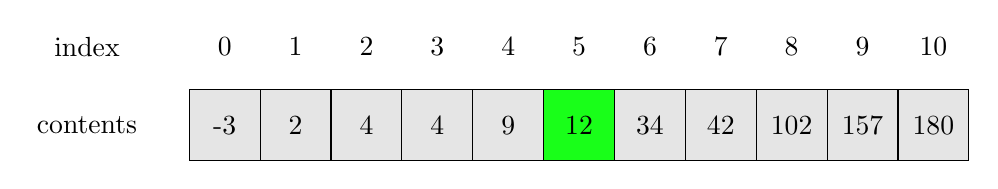
\begin{tikzpicture}
% size of each node
\def\sz{9mm}
% node style definition
\tikzstyle{block} = [
	draw, fill=black!10, rectangle,
	minimum height=\sz, minimum width=\sz ];
\tikzstyle{plain} = [draw=none,fill=none];
% array element definition
\def\arr{0, 2, 4, 4, 9, 12, 34, 42, 102};
%\def\x{0}; % x pos of arr
%\def\y{0}; % y pos of arr
%\newcounter{ind};
%\setcounter{ind}{0};
\node[plain] at (-1.75, 1) { index };
\node[plain] at (-1.75, 0) { contents };

\node[block] at (0,0) { -3 };
\node[plain] at (0,1.0) { 0 };

\node[block] at (1*\sz,0) { 2 };
\node[plain] at (1*\sz,1.0) { 1 };

\node[block] at (2*\sz,0) { 4 };
\node[plain] at (2*\sz,1.0) { 2 };

\node[block] at (3*\sz,0) { 4 };
\node[plain] at (3*\sz,1.0) { 3 };

\node[block] at (4*\sz,0) { 9 };
\node[plain] at (4*\sz,1.0) { 4 };

\node[block,fill=white!10!green] at (5*\sz,0) { 12 };
\node[plain] at (5*\sz,1.0) { 5 };

\node[block] at (6*\sz,0) { 34 };
\node[plain] at (6*\sz,1.0) { 6 };

\node[block] at (7*\sz,0) { 42 };
\node[plain] at (7*\sz,1.0) { 7 };

\node[block] at (8*\sz,0) { 102 };
\node[plain] at (8*\sz,1.0) { 8 };

\node[block] at (9*\sz,0) { 157 };
\node[plain] at (9*\sz,1.0) { 9 };

\node[block] at (10*\sz,0) { 180 };
\node[plain] at (10*\sz,1.0) { 10 };


%\foreach \item in \arr
%{
%	\node[block] (a\theind) at (\theind*\sz,0) { \item };
%	\node[plain] at (\theind*\sz,1.0) { \theind };
%	\addtocounter{ind}{1};
%}
\end{tikzpicture}

}

\subfigure[Since $64 > 12$, we update our left index variable
$l$ to $m + 1$, thus $l = 6$ and we've eliminated the left half
of the list from consideration.]{

\begin{tikzpicture}
% size of each node
\def\sz{9mm}
% node style definition
\tikzstyle{block} = [
	draw, fill=black!10, rectangle,
	minimum height=\sz, minimum width=\sz ];
\tikzstyle{plain} = [draw=none,fill=none];
% array element definition
\def\arr{0, 2, 4, 4, 9, 12, 34, 42, 102};
%\def\x{0}; % x pos of arr
%\def\y{0}; % y pos of arr
%\newcounter{ind};
%\setcounter{ind}{0};
\node[plain] at (-1.75, 1) { index };
\node[plain] at (-1.75, 0) { contents };

\node[block,pattern=north west lines, pattern color=blue] at (0,0) { -3 };
\node[plain] at (0,1.0) { 0 };

\node[block,pattern=north west lines, pattern color=blue] at (1*\sz,0) { 2 };
\node[plain] at (1*\sz,1.0) { 1 };

\node[block,pattern=north west lines, pattern color=blue] at (2*\sz,0) { 4 };
\node[plain] at (2*\sz,1.0) { 2 };

\node[block,pattern=north west lines, pattern color=blue] at (3*\sz,0) { 4 };
\node[plain] at (3*\sz,1.0) { 3 };

\node[block,pattern=north west lines, pattern color=blue] at (4*\sz,0) { 9 };
\node[plain] at (4*\sz,1.0) { 4 };

\node[block,fill=white!10!green] at (5*\sz,0) { 12 };
\node[plain] at (5*\sz,1.0) { 5 };

\node[block] at (6*\sz,0) { 34 };
\node[plain] at (6*\sz,1.0) { 6 };

\node[block] at (7*\sz,0) { 42 };
\node[plain] at (7*\sz,1.0) { 7 };

\node[block] at (8*\sz,0) { 102 };
\node[plain] at (8*\sz,1.0) { 8 };

\node[block] at (9*\sz,0) { 157 };
\node[plain] at (9*\sz,1.0) { 9 };

\node[block] at (10*\sz,0) { 180 };
\node[plain] at (10*\sz,1.0) { 10 };




%\foreach \item in \arr
%{
%	\node[block] (a\theind) at (\theind*\sz,0) { \item };
%	\node[plain] at (\theind*\sz,1.0) { \theind };
%	\addtocounter{ind}{1};
%}
\end{tikzpicture}

}



\subfigure[Our new middle index is $m = \frac{l+r}{2} = \frac{6+10}{2} = 8$, 
corresponding to the element 102.]{

\begin{tikzpicture}
% size of each node
\def\sz{9mm}
% node style definition
\tikzstyle{block} = [
	draw, fill=black!10, rectangle,
	minimum height=\sz, minimum width=\sz ];
\tikzstyle{plain} = [draw=none,fill=none];
% array element definition
\def\arr{0, 2, 4, 4, 9, 12, 34, 42, 102};
%\def\x{0}; % x pos of arr
%\def\y{0}; % y pos of arr
%\newcounter{ind};
%\setcounter{ind}{0};
\node[plain] at (-1.75, 1) { index };
\node[plain] at (-1.75, 0) { contents };

\node[block,pattern=north west lines, pattern color=blue] at (0,0) { -3 };
\node[plain] at (0,1.0) { 0 };

\node[block,pattern=north west lines, pattern color=blue] at (1*\sz,0) { 2 };
\node[plain] at (1*\sz,1.0) { 1 };

\node[block,pattern=north west lines, pattern color=blue] at (2*\sz,0) { 4 };
\node[plain] at (2*\sz,1.0) { 2 };

\node[block,pattern=north west lines, pattern color=blue] at (3*\sz,0) { 4 };
\node[plain] at (3*\sz,1.0) { 3 };

\node[block,pattern=north west lines, pattern color=blue] at (4*\sz,0) { 9 };
\node[plain] at (4*\sz,1.0) { 4 };

\node[block,pattern=north west lines, pattern color=blue] at (5*\sz,0) { 12 };
\node[plain] at (5*\sz,1.0) { 5 };

\node[block] at (6*\sz,0) { 34 };
\node[plain] at (6*\sz,1.0) { 6 };

\node[block] at (7*\sz,0) { 42 };
\node[plain] at (7*\sz,1.0) { 7 };

\node[block,fill=white!10!green] at (8*\sz,0) { 102 };
\node[plain] at (8*\sz,1.0) { 8 };

\node[block] at (9*\sz,0) { 157 };
\node[plain] at (9*\sz,1.0) { 9 };

\node[block] at (10*\sz,0) { 180 };
\node[plain] at (10*\sz,1.0) { 10 };




%\foreach \item in \arr
%{
%	\node[block] (a\theind) at (\theind*\sz,0) { \item };
%	\node[plain] at (\theind*\sz,1.0) { \theind };
%	\addtocounter{ind}{1};
%}
\end{tikzpicture}

}

\subfigure[Since $64 < 102$, we update the right index variable 
$r$ to $m - 1 = 7$, eliminating the right half of the subarray.]{

\begin{tikzpicture}
% size of each node
\def\sz{9mm}
% node style definition
\tikzstyle{block} = [
	draw, fill=black!10, rectangle,
	minimum height=\sz, minimum width=\sz ];
\tikzstyle{plain} = [draw=none,fill=none];
% array element definition
\def\arr{0, 2, 4, 4, 9, 12, 34, 42, 102};
%\def\x{0}; % x pos of arr
%\def\y{0}; % y pos of arr
%\newcounter{ind};
%\setcounter{ind}{0};
\node[plain] at (-1.75, 1) { index };
\node[plain] at (-1.75, 0) { contents };

\node[block,pattern=north west lines, pattern color=blue] at (0,0) { -3 };
\node[plain] at (0,1.0) { 0 };

\node[block,pattern=north west lines, pattern color=blue] at (1*\sz,0) { 2 };
\node[plain] at (1*\sz,1.0) { 1 };

\node[block,pattern=north west lines, pattern color=blue] at (2*\sz,0) { 4 };
\node[plain] at (2*\sz,1.0) { 2 };

\node[block,pattern=north west lines, pattern color=blue] at (3*\sz,0) { 4 };
\node[plain] at (3*\sz,1.0) { 3 };

\node[block,pattern=north west lines, pattern color=blue] at (4*\sz,0) { 9 };
\node[plain] at (4*\sz,1.0) { 4 };

\node[block,pattern=north west lines, pattern color=blue] at (5*\sz,0) { 12 };
\node[plain] at (5*\sz,1.0) { 5 };

\node[block] at (6*\sz,0) { 34 };
\node[plain] at (6*\sz,1.0) { 6 };

\node[block] at (7*\sz,0) { 42 };
\node[plain] at (7*\sz,1.0) { 7 };

\node[block,fill=white!10!green] at (8*\sz,0) { 102 };
\node[plain] at (8*\sz,1.0) { 8 };

\node[block,pattern=north west lines, pattern color=blue] at (9*\sz,0) { 157 };
\node[plain] at (9*\sz,1.0) { 9 };

\node[block,pattern=north west lines, pattern color=blue] at (10*\sz,0) { 180 };
\node[plain] at (10*\sz,1.0) { 10 };




%\foreach \item in \arr
%{
%	\node[block] (a\theind) at (\theind*\sz,0) { \item };
%	\node[plain] at (\theind*\sz,1.0) { \theind };
%	\addtocounter{ind}{1};
%}
\end{tikzpicture}

}


\subfigure[Here, $l = 6, r = 7$, and so our new middle index is
$m = \lfloor \frac{6 + 7}{2}\rfloor = 6$.  Since $64 > 34$, we 
update our left index variable $l$ to $m+1 = 7$]{

\begin{tikzpicture}
% size of each node
\def\sz{9mm}
% node style definition
\tikzstyle{block} = [
	draw, fill=black!10, rectangle,
	minimum height=\sz, minimum width=\sz ];
\tikzstyle{plain} = [draw=none,fill=none];
% array element definition
\def\arr{0, 2, 4, 4, 9, 12, 34, 42, 102};
%\def\x{0}; % x pos of arr
%\def\y{0}; % y pos of arr
%\newcounter{ind};
%\setcounter{ind}{0};
\node[plain] at (-1.75, 1) { index };
\node[plain] at (-1.75, 0) { contents };

\node[block,pattern=north west lines, pattern color=blue] at (0,0) { -3 };
\node[plain] at (0,1.0) { 0 };

\node[block,pattern=north west lines, pattern color=blue] at (1*\sz,0) { 2 };
\node[plain] at (1*\sz,1.0) { 1 };

\node[block,pattern=north west lines, pattern color=blue] at (2*\sz,0) { 4 };
\node[plain] at (2*\sz,1.0) { 2 };

\node[block,pattern=north west lines, pattern color=blue] at (3*\sz,0) { 4 };
\node[plain] at (3*\sz,1.0) { 3 };

\node[block,pattern=north west lines, pattern color=blue] at (4*\sz,0) { 9 };
\node[plain] at (4*\sz,1.0) { 4 };

\node[block,pattern=north west lines, pattern color=blue] at (5*\sz,0) { 12 };
\node[plain] at (5*\sz,1.0) { 5 };

\node[block,fill=white!10!green] at (6*\sz,0) { 34 };
\node[plain] at (6*\sz,1.0) { 6 };

\node[block] at (7*\sz,0) { 42 };
\node[plain] at (7*\sz,1.0) { 7 };

\node[block,pattern=north west lines, pattern color=blue] at (8*\sz,0) { 102 };
\node[plain] at (8*\sz,1.0) { 8 };

\node[block,pattern=north west lines, pattern color=blue] at (9*\sz,0) { 157 };
\node[plain] at (9*\sz,1.0) { 9 };

\node[block,pattern=north west lines, pattern color=blue] at (10*\sz,0) { 180 };
\node[plain] at (10*\sz,1.0) { 10 };




%\foreach \item in \arr
%{
%	\node[block] (a\theind) at (\theind*\sz,0) { \item };
%	\node[plain] at (\theind*\sz,1.0) { \theind };
%	\addtocounter{ind}{1};
%}
\end{tikzpicture}

}

\subfigure[Since $64 > 42$ we again update our left index variable $l$
to $m + 1 = 8$.]{

\begin{tikzpicture}
% size of each node
\def\sz{9mm}
% node style definition
\tikzstyle{block} = [
	draw, fill=black!10, rectangle,
	minimum height=\sz, minimum width=\sz ];
\tikzstyle{plain} = [draw=none,fill=none];
% array element definition
\def\arr{0, 2, 4, 4, 9, 12, 34, 42, 102};
%\def\x{0}; % x pos of arr
%\def\y{0}; % y pos of arr
%\newcounter{ind};
%\setcounter{ind}{0};
\node[plain] at (-1.75, 1) { index };
\node[plain] at (-1.75, 0) { contents };

\node[block,pattern=north west lines, pattern color=blue] at (0,0) { -3 };
\node[plain] at (0,1.0) { 0 };

\node[block,pattern=north west lines, pattern color=blue] at (1*\sz,0) { 2 };
\node[plain] at (1*\sz,1.0) { 1 };

\node[block,pattern=north west lines, pattern color=blue] at (2*\sz,0) { 4 };
\node[plain] at (2*\sz,1.0) { 2 };

\node[block,pattern=north west lines, pattern color=blue] at (3*\sz,0) { 4 };
\node[plain] at (3*\sz,1.0) { 3 };

\node[block,pattern=north west lines, pattern color=blue] at (4*\sz,0) { 9 };
\node[plain] at (4*\sz,1.0) { 4 };

\node[block,pattern=north west lines, pattern color=blue] at (5*\sz,0) { 12 };
\node[plain] at (5*\sz,1.0) { 5 };

\node[block,pattern=north west lines, pattern color=blue] at (6*\sz,0) { 34 };
\node[plain] at (6*\sz,1.0) { 6 };

\node[block,fill=white!10!green] at (7*\sz,0) { 42 };
\node[plain] at (7*\sz,1.0) { 7 };

\node[block,pattern=north west lines, pattern color=blue] at (8*\sz,0) { 102 };
\node[plain] at (8*\sz,1.0) { 8 };

\node[block,pattern=north west lines, pattern color=blue] at (9*\sz,0) { 157 };
\node[plain] at (9*\sz,1.0) { 9 };

\node[block,pattern=north west lines, pattern color=blue] at (10*\sz,0) { 180 };
\node[plain] at (10*\sz,1.0) { 10 };




%\foreach \item in \arr
%{
%	\node[block] (a\theind) at (\theind*\sz,0) { \item };
%	\node[plain] at (\theind*\sz,1.0) { \theind };
%	\addtocounter{ind}{1};
%}
\end{tikzpicture}

}

\subfigure[Since $l = 8$ and $r = 7$, $l > r$ and the loop terminates, 
resulting in an unsuccessful search.]{

\begin{tikzpicture}
% size of each node
\def\sz{9mm}
% node style definition
\tikzstyle{block} = [
	draw, fill=black!10, rectangle,
	minimum height=\sz, minimum width=\sz ];
\tikzstyle{plain} = [draw=none,fill=none];
% array element definition
\def\arr{0, 2, 4, 4, 9, 12, 34, 42, 102};
%\def\x{0}; % x pos of arr
%\def\y{0}; % y pos of arr
%\newcounter{ind};
%\setcounter{ind}{0};
\node[plain] at (-1.75, 1) { index };
\node[plain] at (-1.75, 0) { contents };

\node[block,pattern=north west lines, pattern color=blue] at (0,0) { -3 };
\node[plain] at (0,1.0) { 0 };

\node[block,pattern=north west lines, pattern color=blue] at (1*\sz,0) { 2 };
\node[plain] at (1*\sz,1.0) { 1 };

\node[block,pattern=north west lines, pattern color=blue] at (2*\sz,0) { 4 };
\node[plain] at (2*\sz,1.0) { 2 };

\node[block,pattern=north west lines, pattern color=blue] at (3*\sz,0) { 4 };
\node[plain] at (3*\sz,1.0) { 3 };

\node[block,pattern=north west lines, pattern color=blue] at (4*\sz,0) { 9 };
\node[plain] at (4*\sz,1.0) { 4 };

\node[block,pattern=north west lines, pattern color=blue] at (5*\sz,0) { 12 };
\node[plain] at (5*\sz,1.0) { 5 };

\node[block,pattern=north west lines, pattern color=blue] at (6*\sz,0) { 34 };
\node[plain] at (6*\sz,1.0) { 6 };

\node[block,pattern=north west lines, pattern color=blue] at (7*\sz,0) { 42 };
\node[plain] at (7*\sz,1.0) { 7 };

\node[block,pattern=north west lines, pattern color=blue] at (8*\sz,0) { 102 };
\node[plain] at (8*\sz,1.0) { 8 };

\node[block,pattern=north west lines, pattern color=blue] at (9*\sz,0) { 157 };
\node[plain] at (9*\sz,1.0) { 9 };

\node[block,pattern=north west lines, pattern color=blue] at (10*\sz,0) { 180 };
\node[plain] at (10*\sz,1.0) { 10 };




%\foreach \item in \arr
%{
%	\node[block] (a\theind) at (\theind*\sz,0) { \item };
%	\node[plain] at (\theind*\sz,1.0) { \theind };
%	\addtocounter{ind}{1};
%}
\end{tikzpicture}

}

\caption[Binary Search Example 1]{The worst case scenario for binary search, 
resulting in an unsuccessful search.  This example is run on a 0-indexed array
with an array of integers of size 11.}
\label{figure:binarySearchExample}

\end{figure}




%\end{document}
